%!TeX spellcheck = en-US
%!TEX root = ../hw3_report.tex
\subsection*{(a)}
The matrix
\begin{equation}
  A = \begin{bmatrix}
    \pi & 1 \\
    0 & \pi + \varepsilon
  \end{bmatrix},
\end{equation}
with $\varepsilon > 0$, has two eigenvalues: $\lambda_{1} = \pi$ and $\lambda_{2} = \pi+\varepsilon$. Let $A = X\, \text{diag}(J_{1},J_{2})\,X^{-1},$ be the Jordan canonical form, with $J_{1} = \lambda_{1}$ and $J_{2} = \lambda_{2}$.

The Jordan canonical form definition gives that
\begin{equation}
  p(A) = X\, \text{diag}(p(J_{1}),p(J_{2}))\,X^{-1}.
\end{equation}
 A simple consequence is
\begin{equation}
  g(A) = X\, \text{diag}(g(\lambda_{1}),g(\lambda_{2}))\,X^{-1} = X\, \text{diag}(p(\lambda_{1}),p(\lambda_{2}))\,X^{-1} = p(A),
\end{equation}
since the polynomial $p$ interpolates the function $g$ in the eigenvalues of $A$, i.e. $p(\lambda_{1}) = g(\lambda_{1})$ and $p(\lambda_{2}) = g(\lambda_{2})$.

Two points defines a unique polynomial of order $1$, thus we may choose a $p$ in $\mathbb{P}^{1}$ and write $p(z) = \alpha + \beta z$. The unknown coefficents are obtianed by solving

\begin{equation}
  \begin{cases}
    \alpha + \beta \lambda_{1} &= g(\lambda_{1})\\
    \alpha + \beta \lambda_{2} &= g(\lambda_{2})
  \end{cases}
  \Leftrightarrow
   \begin{cases}
    \alpha  &= \frac{g(\lambda_{1})\lambda_{2}-g(\lambda_{2})\lambda_{1}}{\lambda_{2}-\lambda_{1}}\\
    \beta  &= \frac{g(\lambda_{2})-g(\lambda_{1})}{\lambda_{2}-\lambda_{1}}
  \end{cases}
\end{equation}


\subsection*{(b)}
Given $g\coloneqq \text{exp}$ we have from $(a)$ and $(b)$ that
\begin{align}
  \label{eq:task6exp}
  p(A)  &= \alpha I + \beta A = \frac{\exp{(\pi)}(\pi + \varepsilon)-\exp{(\pi + \varepsilon)}\pi}{\varepsilon} I + \frac{\exp{(\pi + \varepsilon)}-\exp{(\pi)}}{\varepsilon}A \\
  &= \frac{\exp(\pi)}{\varepsilon}(\varepsilon I+(1 - \exp{(\varepsilon)})(\pi I -A))
\end{align}
\subsection*{(c)}
It is known that the Jordan decomposition is unstable for non-symmetric matrices, as the eigenvalues may lie close to each other. For the given matrix $A$ this can be tuned artificially by setting $\varepsilon=|\lambda_{1}-\lambda_{2}|$. As we see in Figure (to be added, some layout to fix). However, the function \texttt{exp} in Julia is analogous to \texttt{expm} in Matlab, (we compared the resluts for $\varepsilon = 1e-1,\ldots,1e-10$). Using Matlabs \texttt{expm}$(A)$ as reference value, the error from the exact result in (b) also increases as $\varepsilon$. This is most likely due to cancellation.

\begin{figure}
\centering
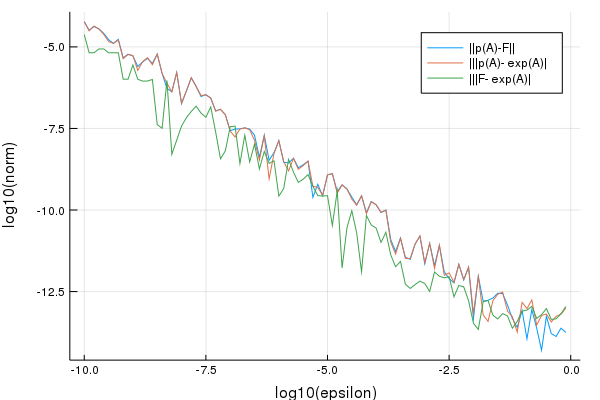
\includegraphics[scale=0.6]{Task6}
\caption{Task $5$, (b) \& (c):  CPU--time in milliseconds, as a function of $N$.}
\label{fig:task6}
\end{figure}
